% 1977 年安徽卷（理科）第 2 题：铁皮槽立体示意图，截面矩形 ABCD（A 左上、B 左下、C 右下、D 右上），
% 槽口两斜棱在远端交汇，其间按原卷标注 π/6 角（按源卷第 2 页「安，二」图布局重绘）
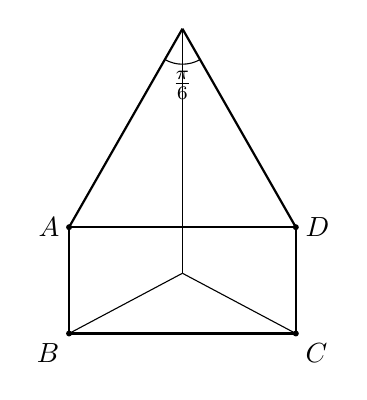
\begin{tikzpicture}[scale=0.9]
  % 前面板矩形
  \coordinate (A) at (0,1.5);
  \coordinate (B) at (0,0);
  \coordinate (C) at (3.2,0);
  \coordinate (D) at (3.2,1.5);
  % 远端顶点（手绘原图将远端上下棱各收缩为一点）
  \coordinate (P) at (1.6,4.3);
  \coordinate (Q) at (1.6,0.85);
  \draw[thick] (A)--(B)--(C)--(D);
  \draw[thick] (A)--(P);
  \draw[thick] (D)--(P);
  \draw[thin]  (B)--(Q);
  \draw[thin]  (C)--(Q);
  \draw[thin]  (P)--(Q);
  \draw[thick] (A)--(D);
  \fill (A) circle (1.2pt) node[left] {$A$};
  \fill (B) circle (1.2pt) node[below left] {$B$};
  \fill (C) circle (1.2pt) node[below right] {$C$};
  \fill (D) circle (1.2pt) node[right] {$D$};
  % 槽口两斜棱夹角标注（原卷标注 π/6，题面与解答未使用，按原样保留）
  \draw (P) ++(240.3:0.5) arc[start angle=240.3, end angle=299.7, radius=0.5];
  \node at (1.6,3.5) {$\frac{\pi}{6}$};
\end{tikzpicture}
